Visualize the elliptic paraboloid $z = x^2/a^2 + y^2/b^2$ for different values of $a > 0$ and $b > 0$.

\begin{solution}\
\begin{lstlisting}
[x, y] = meshgrid(linspace(-10, 10, 100), linspace(-10, 10, 100));
z = x.^2/a^2 + y.^2/b^2;
surf(x, y, z);
shading interp
\end{lstlisting}

With $a > b$:
\begin{center}
    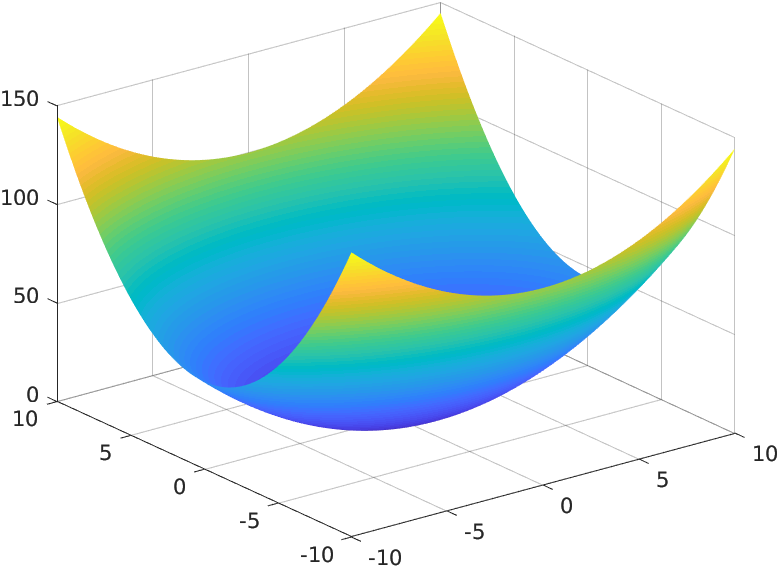
\includegraphics[width=0.5\textwidth]{img/e13p1a.png}
\end{center}

With $a < b$:
\begin{center}
    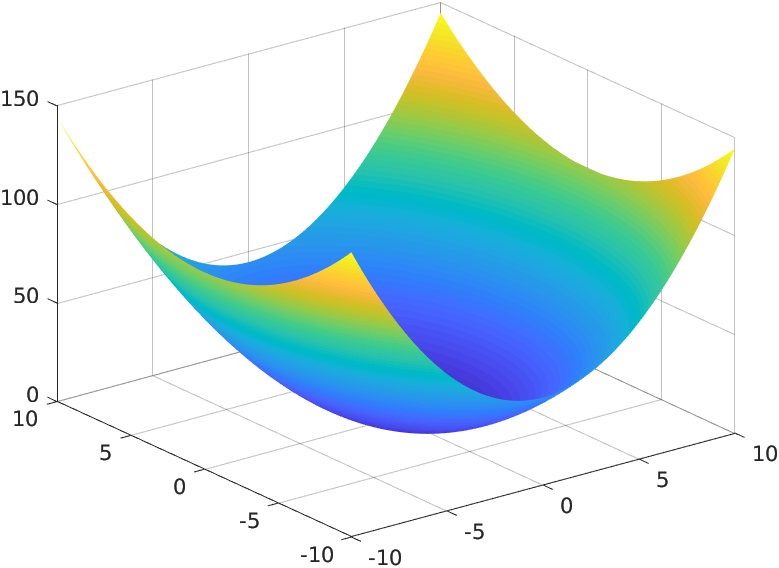
\includegraphics[width=0.5\textwidth]{img/e13p1b.png}
\end{center}
\end{solution}

Describe the contours in the $yz$-plane defined by $x = c$.

\begin{solution}
    This is a parabola that crosses the z-axis at $c^2/a^2$
\end{solution}